\documentclass[12pt,a4paper,openright,twoside]{book}
\usepackage[utf8]{inputenc}
\usepackage{float}

\newcommand{\thesislang}{italian}
\usepackage{thesis-style}
% version
\newcommand{\versionmajor}{0}
\newcommand{\versionminor}{1}
\newcommand{\versionpatch}{2}
\newcommand{\version}{\versionmajor.\versionminor.\versionpatch}
\typeout{Document version: \version}

\begin{document}

\frontmatter

% ! TeX root = thesis-main.tex
\title{Title}
\author{Candidate Name Here}
\date{\today}

\newgeometry{margin=0.8in}
\begin{titlepage}
	\begin{center}
		% \vspace*{0.2cm}

		\Huge
		\vspace{4cm}
		\textbf{
			ChEBI
			\\
			Chemical Entities of Biological Interest
		}

		\large
		\vspace{1cm}
		Elaborato in
		\\
		\textsc{Web Semantico}

		\vspace{5.5cm}
		\begin{minipage}[t]{0.64\textwidth}
			\begin{flushleft}
				\textit{Leonardo Micelli}
				\\
				\textbf{leonardo.micelli@studio.unibo.it}
				\\
				\textbf{0001031320}
				\\
				\vspace{0.4cm}
				\textit{Filippo Vissani}
				\\
				\textbf{filippo.vissani@studio.unibo.it}
				\\
				\textbf{0001026702}
			\end{flushleft}
		\end{minipage}

		\vfill
		\noindent\hrulefill
		\vspace{0.3cm}
		\Large
		\\
		Anno Accademico 2022-2023
	\end{center}
\end{titlepage}
\restoregeometry


%----------------------------------------------------------------------------------------
\tableofcontents
%----------------------------------------------------------------------------------------

\mainmatter

%----------------------------------------------------------------------------------------
\chapter{\introductionname}
\label{chap:introduction}
%----------------------------------------------------------------------------------------

ChEBI (Chemical Entities of Biological Interest) è un'ontologia completa di entità chimiche, con particolare attenzione ai composti chimici "piccoli". Tali entità molecolari, che possono essere
sia naturali che sintetiche, intervengono nei processi biologici degli organismi viventi. ChEBI è progettato per essere utilizzato nell'annotazione e nell'indicizzazione di composti chimici in database e letteratura, nonché nell'analisi di dati chimici.
L'ontologia ChEBI fornisce una classificazione gerarchica delle entità chimiche, basata sulle loro proprietà strutturali e funzionali, nonché sui loro ruoli e applicazioni biologiche. L'ontologia comprende varie classi di composti, come aminoacidi, nucleotidi, lipidi, carboidrati, steroidi e prodotti naturali, nonché composti sintetici e farmaci.
ChEBI contiene informazioni estese sulle proprietà e le attività delle entità chimiche, tra cui le loro strutture chimiche, i pesi molecolari, i punti di fusione, i punti di ebollizione, le solubilità e gli effetti farmacologici.
Le entità presenti in ChEBI sono legate tra loro tramite il concetto di relazione, che definisce la tipologia di legame che c'è tra esse.
ChEBI è disponibile online e può essere consultato tramite il sito web: \url{http://www.ebi.ac.uk/chebi/}.

%----------------------------------------------------------------------------------------
\chapter{Panoramica di ChEBI}
\label{chap:panoramica}
%----------------------------------------------------------------------------------------
L'ontologia ChEBI è una classificazione strutturata delle entità chimiche sopra descritte. La sua struttura è essenzialmente quella di un grafo aciclico direzionato (DAG), in cui le entità chimiche sono i nodi e le relazioni sono gli archi.
Questa struttura differisce da una semplice tassonomia in quanto un nodo figlio può avere molti nodi padre.
La struttura DAG di ChEBI è mostrata nella Figura \ref{fig:Caffeine}.

\begin{figure}[H]
	\centering
	\includegraphics[width=\linewidth]{figures/caffeine.png}
	\caption{Struttura DAG di ChEBI}
	\label{fig:Caffeine}
\end{figure}

L'ontologia è a sua volta suddivisa in tre sotto-ontologie principali: \textit{Chemical Entity}, \textit{Role} e \textit{Subatomic Particle}.

\section{Chemical Entity}

Una \textit{Chemical Entity} è definita come qualsiasi entità molecolare, sia essa sintetica o di origine naturale, che ha una struttura chimica ben definita ed è in grado di interagire con i sistemi biologici.

In ChEBI, i le entità chimiche sono suddivise in quattro sotto-categorie principali:
\begin{itemize}
	\item \textit{Group}: è un insieme di entità chimiche che hanno una struttura chimica comune.
	\item \textit{Molecular Entity}: è un insieme di atomi che sono legati tra loro da legami chimici.
	\item \textit{Atom}: è l'unità minima di materia che non può essere ulteriormente divisa senza perdita di identità.
	\item \textit{Chemical Substance}: è una sostanza chimica che ha una composizione chimica ben definita.
\end{itemize}


\begin{figure}[H]
	\centering
	\includegraphics[width=\linewidth]{figures/chemical-entity.png}
	\caption{Gerarchia più esterna di chemical entity}
	\label{fig:ChemicalEntity}
\end{figure}
\section{Role}
Un \textit{Role} è una funzione o un compito che una entità chimica può svolgere. Un ruolo può essere svolto da una singola entità chimica o da un gruppo di entità chimiche. In ChEBI, i ruoli sono suddivisi in tre sotto-categorie principali:
\begin{itemize}
	\item \textit{Biological Role}: è un ruolo che una entità chimica può svolgere in un organismo vivente.
	\item \textit{Chemical Role}: è un ruolo che una entità chimica può svolgere in un composto chimico.
	\item \textit{Application}: è un ruolo che una entità chimica può svolgere in un processo industriale o in un'attività umana.
\end{itemize}

\begin{figure}[H]
	\centering
	\includegraphics[width=\linewidth]{figures/role.png}
	\caption{Gerarchia più esterna di role}
	\label{fig:Role}
\end{figure}

\section{Subatomic Particle}
Una \textit{Subatomic Particle} è una particella più piccola di un atomo.
In ChEBI, le particelle subatomiche sono suddivise nelle seguenti sotto-categorie principali:
\begin{itemize}
	\item \textit{Boson}: è una particella subatomica responsabile delle interazioni fondamentali e del fenomeno della massa.
	\item \textit{Composite Particle}: è una particella subatomica che è costituita da più di un quark.
	\item \textit{Fermion}: è una particella subatomica che ha una massa non nulla e che interagisce solo con altre particelle subatomiche.
	\item \textit{Fundamental Particle}: è una particella subatomica che non può essere ulteriormente divisa senza perdita di identità.
	\item \textit{Nuclear Particle}: è una particella subatomica che costituisce il nucle di un atomo.
\end{itemize}

\begin{figure}[H]
	\centering
	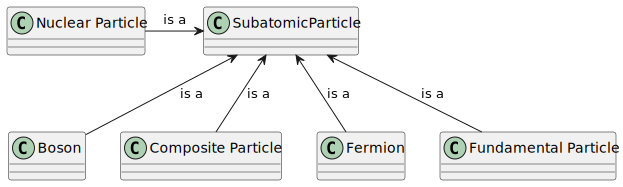
\includegraphics[width=\linewidth]{figures/subatomic-particle.png}
	\caption{Gerarchia più esterna di subatomic particle}
	\label{fig:SubatomicParticle}
\end{figure}

%----------------------------------------------------------------------------------------
\chapter{Esempi di Risorse}
\label{chap:classexamples}

In ChEBI le risorse, cioè i componenti che costituiscono i nodi del grafo, possono avere vari attributi, tra i quali:
\begin{itemize}
	\item \textit{Definition}: descrizione della risorsa.
	\item \textit{ID}: Identificatore univoco della risorsa.
	\item \textit{Name}: Nome della risorsa.
	\item \textit{Star}: Numero di stelle che la risorsa ha ricevuto.
	\item \textit{Formula}: Formula chimica della risorsa.
\end{itemize}

In Figura \ref{fig:Class} è mostrato un esempio di risorsa.

\begin{figure}[H]
	\centering
	\includegraphics[width=\linewidth]{figures/class.png}
	\caption{Esempio di classe}
	\label{fig:Class}
\end{figure}

Nel listato \ref{lst:caffeine} è mostrato un esempio di risorsa utilizzando il linguaggio OWL.

\lstinputlisting[
	float,
	language=XML,
	caption={OWL class for caffeine},
	label={lst:caffeine},
]{listings/caffeine.xml}

%----------------------------------------------------------------------------------------
\chapter{Relazioni}
\label{chap:relationships}
%----------------------------------------------------------------------------------------

In ChEBI le classi sono legate tra loro tramite relazioni. Le relazioni sono:
\begin{itemize}
	\item \textit{is a}: indica che una classe è una sottoclasse di un'altra classe.
	\item \textit{has role}: indica che una classe ha un ruolo.
	\item \textit{has part}: indica una relazione tra un insieme e le sue parti.
	\item \textit{is a conjugate base of}: indica che una classe è una base coniugata di un'altra. classe.
	\item \textit{is a conjugate acid of}: indica che una classe è un acido coniugato di un'altra classe.
	\item \textit{is tautomer of}: indica che una classe è un tautomero di un'altra classe.
	\item \textit{is enantiomer of}: indica che una classe è un enantiomero di un'altra classe.
	\item \textit{has functional parent}: indica che una classe ha un genitore funzionale.
	\item \textit{has parent hydride}: indica che una classe ha un genitore idride.
	\item \textit{is substituent group of}: indica che una classe è un gruppo sostitutivo di un'altra classe.
\end{itemize}

Alle relazioni viene anche associato un simbolismo ben definito, il quale viene presentato in Figura \ref{fig:RelationshipTypes}.

\begin{figure}[H]
	\centering
	\includegraphics[width=\linewidth]{figures/relationship-types.png}
	\caption{Esempio di classe}
	\label{fig:RelationshipTypes}
\end{figure}

%----------------------------------------------------------------------------------------
\chapter{Progetti}
\label{chap:projects}
%----------------------------------------------------------------------------------------
\section{ChEMBL}
ChEMBL è un database che contiene informazioni sulle proprietà dei composti chimici utilizzati nella ricerca di nuovi farmaci. ChEBI viene utilizzato in ChEMBL per fornire informazioni sulle entità chimiche che vengono studiate. Ciò aiuta i ricercatori a identificare i composti chimici che potrebbero avere proprietà farmacologiche desiderate, come la capacità di legarsi a specifiche proteine o di avere attività biologica specifica.

\section{DrugBank}
Il progetto DrugBank è un database online che raccoglie informazioni sulle droghe e sui loro bersagli molecolari. Il database è stato creato nel 2006 presso l'Università dell'Alberta, in Canada, e fornisce informazioni su oltre 12.000 farmaci e composti bioattivi.

Le informazioni contenute in DrugBank includono la struttura chimica delle droghe, i loro meccanismi d'azione, gli effetti collaterali, le interazioni farmacologiche e le vie metaboliche che le droghe seguono nel corpo. Inoltre, il database fornisce informazioni sulle proteine e sui loro bersagli molecolari che sono coinvolti nei processi fisiologici, sui quali agiscono i farmaci.

Il progetto DrugBank ha l'obiettivo di fornire informazioni accurate e aggiornate sui farmaci per aiutare i professionisti sanitari, i ricercatori e il pubblico in generale a comprendere meglio l'efficacia e la sicurezza delle droghe.

\paragraph{} In ChEBI, le droghe possono essere modellate attraverso le loro entità costituenti e le relazioni 'is a', 'has role', 'has part' ed 'is enantiomer of';
dunque ad una particolare entry di DrugBank corrisponde una porzione di grafo di ChEBI.

È possibile accedere al database, disponibile in formato XML ed RDF, su \url{https://go.drugbank.com/}.

\section{Neuroscience Information Framework}
Il Neuroscience Information Framework è un repository di risorse web globali di neuroscienze, inclusi database di neuroscienze sperimentali, clinici e traslazionali, basi di conoscenza, atlanti e risorse genetiche/genomiche e fornisce molti collegamenti autorevoli in tutto il portale di neuroscienze di Wikipedia.
A differenza dei motori di ricerca generici, NIF fornisce un accesso molto più profondo a un insieme mirato di risorse rilevanti per le neuroscienze, strategie di ricerca su misura per le neuroscienze e accesso a contenuti che sono tradizionalmente "nascosti" dai motori di ricerca web.
Il NIF è un inventario dinamico di database di neuroscienze, annotato e integrato con un sistema unificato di terminologia biomedica (es. NeuroLex).
NIF supporta query basate su concetti su più scale di struttura biologica e più livelli di funzione biologica, semplificando la ricerca e la comprensione dei risultati.
Uno degli obiettivi futuri di NIF sarà fornire anche un registro attraverso il quale i fornitori di risorse possono rivelare la disponibilità di risorse rilevanti per la ricerca neuroscientifica. NIF non intende essere un magazzino o un deposito in sé, ma un mezzo per divulgare e localizzare risorse altrove disponibili tramite il web.

\paragraph{} In questo progetto, ChEBI viene utilizzato per modellare le entità chimiche che sono oggetto di studio, come ad esempio i composti chimici che sono stati utilizzati per studiare il comportamento di un particolare neurone.
Quando gli scienziati inseriscono dati nel NIF, utilizzano ChEBI per classificare le sostanze chimiche coinvolte in quei dati.
Ad esempio, se un ricercatore inserisce dati sulle interazioni proteina-sostanza chimica, utilizza ChEBI per descrivere la sostanza chimica coinvolta.
ChEBI è utilizzato per standardizzare la descrizione delle sostanze chimiche in modo che gli scienziati possano facilmente trovare informazioni su di esse e confrontarle tra loro.

%----------------------------------------------------------------------------------------
\chapter{Conclusioni}
\label{chap:conclusions}
%----------------------------------------------------------------------------------------
In questa ricerca abbiamo introdotto ChEBI, un'ontologia che si prefissa di modellare le entità chimiche di interesse biologico. Abbiamo proceduto a fare una panoramica della sua struttura, composta da tre sotto-ontologie, ognuna con il proprio specifico obiettivo. Siamo passati a definire le possibili relazioni tra i concetti presenti in ChEBI, grazie alle quali è possibile modellare risorse in maniera completa ed efficace (come si è potuto apprezzare nel listato \ref{lst:caffeine}).

Dato il dominio nel quale si colloca, ChEBI è particolarmente adatta a progetti in contesti affini alla biologia come healthcare e, soprattutto, la farmacologia.

In conclusione, riteniamo che ChEBI sia uno strumento molto utile per modellare la conoscenza in qualsiasi ambito bio-chimico, grazie anche alla sua semplicità.


\end{document}